\documentclass[../masters.tex]{subfiles}

\begin{document}
\graphicspath{{./imgs/}{../imgs/}} %look for images

\section{Linear Models}
In this section we consider probabilistic graphical models of the form shown in Figure \ref{fig_linmod}. This model is a generalisation of the graphical model seen in the Hidden Markov Model section. We now assume that the states ($X = x_1,x_2,...$) and observations ($Y=y_1,y_2,...$) are continuous random variables but the inputs ($U=u_1,u_2,...$) are deterministic. Models of this form are called Latent Linear Dynamical Systems (the famous Kalman Filter model falls into this category).
\begin{figure}[H] 
\centering
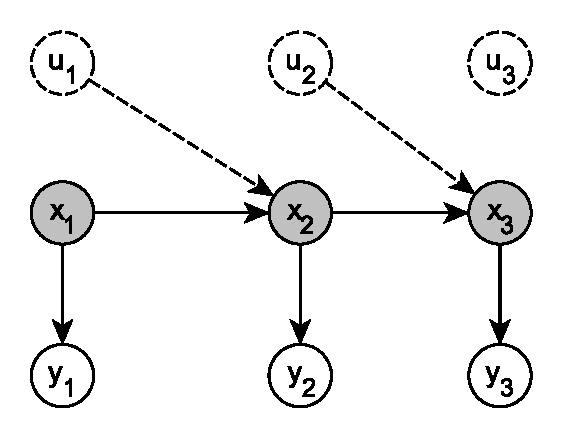
\includegraphics[scale=1.0]{linear_model.pdf}
\caption{Graphical model of this section}
\label{fig_linmod}
\end{figure}
In the previous section we developed inference algorithms but assumed that the transition and observation functions were discrete. We also noted that this assumption is not appropriate for continuous data. The reason is that one would invariably need to discretise the domain of the continuous random variable under consideration. This would result in intractably large discrete systems if one requires fine resolution. To address this issue we extend the previous model to include both continuous states and observations. 

We assume linearity and that all the random variables are Gaussian. While these are strong assumptions they form the building blocks of much more expressive models as we will discover in the next section. We also assume that the transition and emission functions are time invariant. The state space model is of the form (\ref{eq_statespace}).
\begin{equation}
\begin{aligned}
x_{t+1} &= Ax_t + Bu_t + w_{t+1} \text{ with } \mathcal{N}(w_{t+1}|0,Q) \\
y_{t+1} &= Cx_{t+1} + v_{t+1}  \text{ with } \mathcal{N}(v_{t+1}|0,R)
\end{aligned}
\label{eq_statespace}
\end{equation}
Rewriting the state space model we see that the transition and emission functions are given by (\ref{eq_trans_emiss}). Note that we also assume that the system is first order Markov.
\begin{equation}
\begin{aligned}
p(x_{t+1}|x_t, u_t)&= \mathcal{N}(x_{t+1}|Ax_t+Bu_t, Q) \\
p(y_{t+1}|x_t) &= \mathcal{N}(y_{t+1}|Cx_{t+1}, R)
\end{aligned}
\label{eq_trans_emiss}
\end{equation}
We have implicitly assumed that the noise is Gaussian and white\footnote{The noise is temporally independent, has zero mean and finite variance.}. Intuitively one can think of $R$ being the covariance of the noise associated with state measurements and $Q$ being the uncertainty (plant-model mismatch) associated with the linear model of the plant. Additionally, $Q$ can also model any unmeasured disturbances which may influence the system\footnote{Note that for the purposes of this dissertation plant is a synonym for the system.}. Thus, larger $R$ and $Q$ indicate more uncertainty in the system. 

\subsection{Filtering}
The goal of filtering is to find the posterior distribution $p(x_{t}|y_{1:t}, u_{1:t-1})$. It is pleasing to note that this derivation will follow in an analogous manner to the filtering derivation in the Hidden Markov Model section albeit with continuous Gaussian distributions. Thus, the motivation for taking the joint of only the preceding hidden time step is the same. We start with the prediction expression in (\ref{eq_filter_pred}) and assume, due to the closure of linear conditional Gaussian distributions, that $\alpha(x_{t-1}) = p(x_{t-1}|y_{1:t-1}, u_{1:t-2}) = \mathcal{N}(x_{t}|\mu_t, \Sigma_t) $. 
\begin{equation}
\begin{aligned}
p(x_t|y_{1:t-1}, u_{1:t-1}) &= \int p(x_t,x_{t-1}|y_{1:t-1}, u_{1:t-1}) dx_{t-1} \\
&= \int p(x_{t-1}|y_{1:t-1}, u_{1:t-1})p(x_{t}|x_{t-1}, y_{1:t-1}, u_{1:t-1}) dx_{t-1} \\
&= \int p(x_{t-1}|y_{1:t-1}, u_{1:t-2})p(x_{t}|x_{t-1}, u_{1:t-1}) dx_{t-1} \\
&= \int \alpha(x_{t-1})\mathcal{N}(x_{t}|Ax_{t-1}+Bu_{t-1}, Q) dx_{t-1} \\
&= \int \mathcal{N}(x_{t-1}|\mu_{t-1}, \Sigma_{t-1}) \mathcal{N}(x_{t}|Ax_{t-1}+Bu_{t-1}, Q) dx_{t-1} \\
\end{aligned}
\label{eq_filter_pred}
\end{equation} 
Now we use Bayes' Theorem for Linear Gaussian Models to evaluate the marginal expression as shown in ().
\begin{equation}
\int \mathcal{N}(x_{t-1}|\mu_{t-1}, \Sigma_{t-1}) \mathcal{N}(x_{t}|Ax_{t-1}+Bu_{t-1}, Q) dx_{t-1}
\end{equation}



\bibliographystyle{plain}
\bibliography{research}

\end{document}